%%%  default
\documentclass[10pt, compress]{beamer}


\usetheme{mnuig}
\usepackage{tikz}
\usepackage{booktabs}
%\usepackage{cite}
\bibliographystyle{apalike}

%\usepackage[scale=2]{ccicons}

%\usemintedstyle{trac}
\usepackage{grffile} %for underscores in file names

\title{GRC Meeting: 2016 - 2017}
\subtitle{Comparative Genomics of Soil-adapted \textit{E. coli}}
\date{\footnotesize{\today}}
\author{\\ \\ \\ \\Nick Waters}
\institute{Department of Microbiology\\
School of Natural Sciences\\
National University of Ireland, Galway}

%%%%% %%%%% %%%%% %%% %%%%  for pretty headers with pictures
\addtobeamertemplate{frametitle}{}{%
\begin{tikzpicture}[remember picture,overlay]
\node[anchor=north east,yshift=2pt] at (current page.north east) {
\includegraphics[height=0.8cm]{../stock_logos/nuig_rounded.png}  \hspace*{.05cm} 
\includegraphics[height=.794cm, trim= 0cm 0.0cm 0.0cm 0cm]{../stock_logos/jhi_rounded.png}};
\end{tikzpicture}}




\begin{document}

\maketitle

\section{Overview}

\begin{frame}[fragile]
  \frametitle{Outline}
  \begin{itemize}
  \item Genome Assembly
  \item Phylogenetics, MLST, and Collection Overview
  \item Virulence
  \item Plans
    \end{itemize}
\end{frame}

\section{Genome Assembly}

\begin{frame}[fragile]
  \frametitle{State of Available Bacterial Genomes}
\begin{table}[]
\centering
\caption{Bacterial Genome Completion as of 4/1/17}
\label{my-label}
\begin{tabular}{l|llll}
  Total & Complete genome & Chromosome & Contig & Scaffold \\
  \hline\\
85799 & 6255            & 1143       & 38429  & 39972
\end{tabular}
\end{table}
\vspace{2cm}
\end{frame}



\begin{frame}[fragile]
  \frametitle{State of Sequencing Data Availability}
\begin{table}[]
\centering
\caption{Hits per Search Term in NCBI's SRA}
\label{my-label}
\begin{tabular}{l|ll}
  Search term & hits    & percentage \\
  \hline\\
'illumina'    & 2242225 & (94.27)      \\
'pacbio'      & 21131   & (0.89)       \\
'ion'         & 30560   & (1.28)     \\
'roche'     & 42445   & (1.78)       \\
'oxford'      & 12301   & (0.52)       \\
'solid'       & 29791   & (1.25)       \\
            &         &            \\
Total       & 2378453 & (100)
\end{tabular}
\end{table}
\end{frame}


\begin{frame}[fragile]
  \frametitle{Improving Illumina Short Read Assembly}
\begin{enumerate}
\item Within a taxonomic group, GC content is largely conserved.
\item Within a taxonomic group, genome size is largely conserved.
\item Bacterial genomes are dense.
\item Nucleotide order is not random.
\end{enumerate}

\end{frame}

\begin{frame}[fragile]
  \frametitle{riboSeed}
    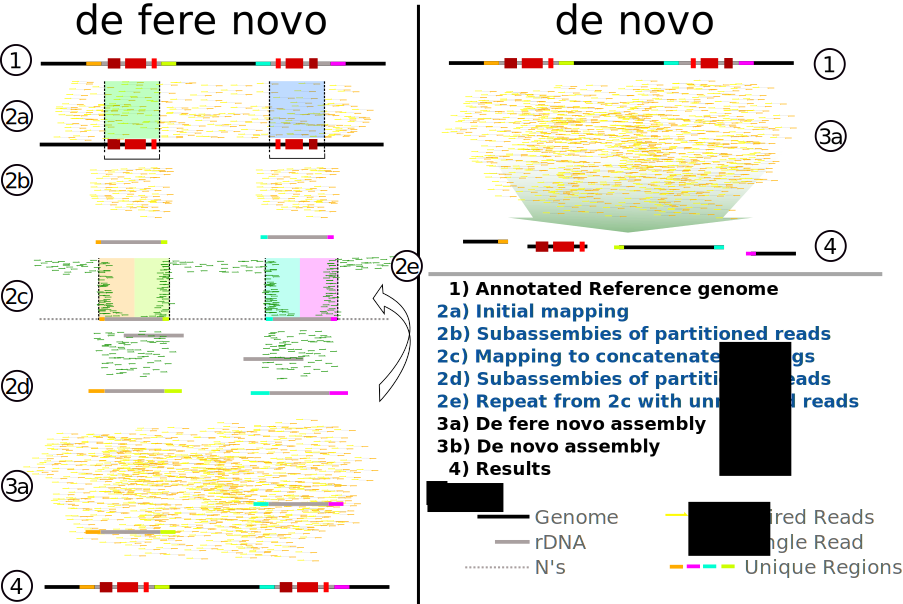
\includegraphics[width=\textwidth]{../../notebook/figures/riboSeed/riboSeed_v8.png}\\

\end{frame}


\begin{frame}[fragile]
  \frametitle{Benchmarking riboSeed}
\begin{itemize}
\item Simulated Reads on a Simulated Genome
\item Simulated Reads on Real Genomes
\item Hybrid Assembly Validation
\item GAGE-B Dataset
\end{itemize}

\end{frame}


\begin{frame}[fragile]
  \frametitle{Benchmarking: Simulated Genome}
    \includegraphics[width=\textwidth]{~/GitHub/riboSeed/manuscript_figs/mauve.png}\\
\end{frame}


\begin{frame}[fragile]
  \frametitle{Benchmarking: Simulated Reads on Sakai}
  \begin{table}[]
    % \resizebox{\textwidth}{!}
\centering
\caption{riboSeed on simulated Sakai reads }
\label{my-label}
\begin{tabular}{llll}
  Coverage &Ref. rDNAs& De novo(skip, miss)&De fere novo (skip, miss) \\
  \hline\\
  10&   7&      0 (7, 0)&	3 (4, 0)\\
  20&	7&	0 (7, 0)&	6 (1, 0)           \\
  50&	7&	0 (7 , 0)&	6 (1, 0)           \\
  100&	7&	0 (7 , 0)&	6 (1, 0)\\
\end{tabular}

\end{table}
\end{frame}


\begin{frame}[fragile]
  \frametitle{Benchmarking: Hybrid Assembly}
\begin{table}[]
\centering
\caption{riboSeed on Pseudomonas aeruginosa strain BAMCPA07-48 }
\begin{tabular}{llll}
  Coverage & Re. rDNA &	De novo (skip, miss) &	De fere novo (skip, miss)   \\
  \hline
  200    & 4  & 1(3, 0)  & 4(0, 0)  \\
\end{tabular}
\end{table}
\end{frame}




\begin{frame}[fragile]
  \frametitle{riboSeed: next steps}
  \begin{itemize}
  \item Finish benchmarking
  \item  Applicability to fungal and archaeal genomes
  \item Improve Signal-to-noise ratio
  \end{itemize}
\end{frame}



%%%%%%%%%%%%%%%%%%%%%%%%%%%%%%%%%%%%%%%%%%%%%%%%%%%%%%%%%%%%%%%%%%%%
\section{Aggregating Metadata}
\begin{frame}[fragile]
  \frametitle{ Experimental Metadata}
  Problem: lack of single repository for the data related to the collection
  \begin{itemize}
  \item Sample Isolation data
  \item Phenotypic tests
    \item Phylotyping
  \end{itemize}
\end{frame}

\begin{frame}[fragile]
  \frametitle{In silico  Metadata}
  \begin{itemize}
  \item Library preparataion and sequencing QC
  \item Average nucleotide identity
  \item In silico Clermont PCR
  \item MLST
    \end{itemize}
\end{frame}

\begin{frame}[fragile]
  \frametitle{Results and Implications}
  After eliminating isolates falling beneath the 95\% ANI threshold and those with poor sequencing data, the collection consists of 153 isolates.
  \begin{itemize}
  \item Prevents duplication of work
  \item Aids automation
  \item Allows investigation of meta-variables
    \end{itemize}
\end{frame}


\section{Preliminary Virulence Profiling}

\begin{frame}[fragile]
  \frametitle{Virulence}

  \begin{itemize}
  \item Search literature for genes implicated in virulence
  \item Select representative sequences for ~50 virulence factors
  \item Use reciprocal translated blast to find occurrences
  \item Filter results, visualize
  \end{itemize}
\end{frame}

\begin{frame}<1>[label=zooms]
  \frametitle<1>{Virulence}
  \framezoom<1><2>[border](4.2cm,6cm)(2cm,2cm)
  % \framezoom<1><3>[border](1cm,3cm)(2cm,1.5cm)
    \pgfimage[height=8cm]{../../posters/utrecht2016/figs/20161122170535_blast_virulence_parser_output_heatmap_edited3.pdf}
  \end{frame}
%  this controls the zoomed slides
  \againframe<2->[plain]{zooms}

\begin{frame}[fragile]
  \frametitle{Virulence: Next Steps}
  \begin{itemize}
  \item Compare with recent tools (ARIBA, VirulenceFinder, etc)
  \item Experimentally assess phenotypes as needed
  \end{itemize}
\end{frame}
\section{Plans for 2017-2018}
\begin{frame}[fragile]
  \frametitle{Future Work}
  riboSeed development:
  \begin{itemize}
  \item Improve progressive QC to identify problems early
  \item Investigate characteristics of rDNAs that may be predictive of riboSeed success
  % \item Implement for other repeated genomic features
  \end{itemize}
  Exploring the E. coli pangenome:
  \begin{itemize}
  \item Attempt to isolate genomic trends indicative of soil-adaptation
  \item Establish pangenomic context of the the collection
  \item Correlate metadata with pangenome
  \end{itemize}
  Curli loss:
  \begin{itemize}
  \item Utilize phenotypic data from Y. Soronin and others to determine additional causes of curli loss
  \end{itemize}


\end{frame}



\begin{frame}{Acknowledgments}
  \begin{columns}[onlytextwidth]
    \column{0.5\textwidth}
    \includegraphics[height=1cm]{../stock_logos/NUI_Galway_BrandMark_A_K.eps}\\
     NUIG Microbiology
      \begin{itemize}
        \item Dr. Fiona Brennan
        \item Dr. Florence Abram
        \item Matthias Waibel
        \item Stephen Nolan
        \item Camilla Thorn
      \end{itemize}

    \column{0.5\textwidth}
    
\includegraphics[height=1cm]{../stock_logos/trimmed_jhi.png}\\
      James Hutton Institute, Dundee
      \begin{itemize}
        \item Dr. Leighton Pritchard
        \item Dr. Ashleigh Holmes
      \end{itemize}
  \end{columns}
\end{frame}



\plain{}{Questions?}

\end{document}
